\scalebox{1.2}{
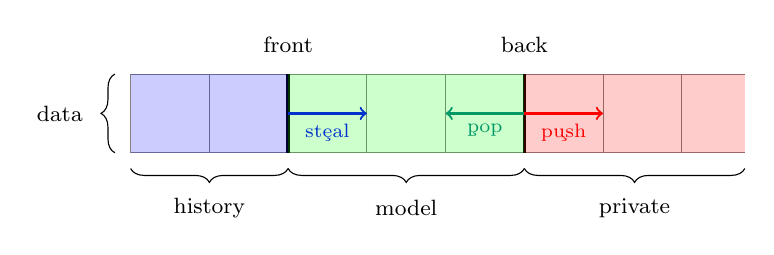
\begin{tikzpicture}
  \def\history{2}
  \def\model{3}
  \def\private{2.8}

  \visible<1->{
    \draw [step=1cm, gray] (0,0) grid ++(\history+\model+\private,1) ;
    \draw [decorate, decoration={brace, amplitude=5pt}] (-.2,0) -- ++(0,1) node [midway, xshift=-7mm] {\footnotesize data} ;
  }

  \visible<2->{
    \draw [very thick] (\history,0) -- ++(0,1) node [label=above:\footnotesize front] {} ;
    \draw [thick, ->, blue] (\history,.5) -- ++(1,0) node [midway, below] {\scriptsize\c{steal}} ;
  }
  
  \visible<3->{
    \draw [very thick] (\history+\model,0) -- ++(0,1) node [label=above:\footnotesize back] {} ;
    \draw [thick, ->, teal] (\history+\model,.5) -- ++(-1,0) node [midway, below] {\scriptsize\c{pop}} ;
    \draw [thick, ->, red] (\history+\model,.5) -- ++(1,0) node [midway, below] {\scriptsize\c{push}} ;
  }
  
  \visible<4->{
    \fill [blue, opacity=.2] (0,0) rectangle ++(\history,1) ;
    \draw [decorate, decoration={brace, amplitude=5pt}] (\history,-.2) -- ++(-\history,0) node [midway, yshift=-5mm] {\footnotesize history} ;
  }
  
  \visible<5->{
    \fill [green, opacity=.2] (\history,0) rectangle ++(\model,1) ;
    \draw [decorate, decoration={brace, amplitude=5pt}] (\history+\model,-.2) -- ++(-\model,0) node [midway, yshift=-5mm] {\footnotesize model} ;
  }
  
  \visible<6->{
    \fill [red, opacity=.2] (\history+\model,0) rectangle ++(\private,1) ;
    \draw [decorate, decoration={brace, amplitude=5pt}] (\history+\model +\private,-.2) -- ++(-\private,0) node [midway, yshift=-5mm] {\footnotesize private} ;
  }
\end{tikzpicture}
}

\vfill

\begin{tabular}{r@{:\hskip1em}l}
  \visible<1->{
      data &
      infinite array storing all values
  }
  \visible<2->{
    \\
      front &
      \emph{monotonic} thieves' index
  }
  \visible<3->{
    \\
      back &
      owner's index
  }
  \visible<4->{
    \\
      history &
      \emph{monotonic} list of values
  }
  \visible<5->{
    \\
      model &
      logical content of the deque
  }
  \visible<6->{
    \\
      private &
      owner-only region
  }
\end{tabular}
